% ==============================================================================
% MODULE 02: LITERATURE SURVEY AND BACKGROUND STUDY
% ==============================================================================

\chapter{Literature Survey and Background Study}
\label{chap:literature_survey}

The design of modern video delivery systems represents an intricate balance between infrastructure expenditure, content discovery, network topology, and end-user quality of experience (QoE). This chapter presents a rigorous critical review of the existing technological landscape, categorizing prior work into centralized cloud video-on-demand (VOD) architectures, self-hosted edge media systems, and peer-to-peer (P2P) decentralized distribution networks. Furthermore, it establishes the theoretical underpinnings of hardware-accelerated video coding, adaptive segment delivery, and reverse proxy NAT traversal that underpin the CustardFin architecture.

% ------------------------------------------------------------------------------
\section{Analysis of Centralized Cloud Video Platforms}
\label{sec:survey_centralized}
% ------------------------------------------------------------------------------

Centralized cloud video platforms, typified by YouTube, Vimeo, Netflix, and enterprise architectures built upon hyperscale cloud providers (such as Amazon Web Services Media Services, Google Cloud Video Intelligence, and Microsoft Azure Media Services), rely on complete cloud-side custody of media assets \cite{armbrust2010view}. 

\subsection{Architectural Pipeline}
The standard centralized ingestion and distribution pipeline proceeds through four distinct operational phases, as illustrated mathematically:
\begin{enumerate}
    \item \textbf{Binary Upload and Staging:} The content producer transmits the monolithic raw or pre-compressed master video binary (typically ProRes, DNxHD, or high-bitrate MP4) over HTTP/S or FTP to cloud object storage (e.g., Amazon S3 or Google Cloud Storage).
    \item \textbf{Centralized Distributed Transcoding:} Cloud compute clusters (e.g., AWS Elemental MediaConvert or elastic pools of GPU-enabled EC2 instances) ingest the master binary. They decompress and re-encode the source into multi-bitrate profiles (such as 1080p at 5.0~Mbps, 720p at 2.8~Mbps, and 480p at 1.2~Mbps) formatted as fragmented MP4 or MPEG-TS segments with corresponding HTTP Live Streaming (HLS) or Dynamic Adaptive Streaming over HTTP (DASH) manifests.
    \item \textbf{Permanent Redundant Storage:} All multi-bitrate renditions, manifests, and audio tracks are persisted indefinitely in cloud object storage buckets with $99.999999999\%$ (11 nines) durability guarantees across multiple availability zones.
    \item \textbf{Global Content Delivery Network (CDN) Edge Delivery:} Geographically dispersed points of presence (PoPs) cache media segments at the network edge, terminating TLS sessions close to the viewer and serving chunk requests with low round-trip latency.
\end{enumerate}

\subsection{Economic and Operational Inefficiencies}
While centralized platforms deliver exceptional playback reliability and global scalability, their economic model is fundamentally prohibitive for independent creators, self-hosters, and non-commercial educational organizations:
\begin{itemize}
    \item \textbf{Linear Storage Cost Accumulation:} In standard cloud object storage, pricing scales linearly with total library volume, regardless of viewership activity \cite{aws2024s3pricing}. For standard tiers (e.g., AWS S3 Standard at \$0.023 or \rupee~1.932 per gigabyte-month), a modest collective catalog of $100\text{ TB}$ incurred by a small community incurs a non-negotiable monthly storage fee:
    \begin{equation}
        C_{\text{storage}} = 100{,}000\text{ GB} \times \text{\rupee~1.932/\text{GB-month}} = \text{\rupee~1{,}93{,}200/month} \quad (\text{\rupee~23.18 Lakhs/year})
    \end{equation}
    This cost is incurred perpetually, even for long-tail, archival, or personal media that is viewed only once a year.
    \item \textbf{Asymmetric Data Egress Penalties:} Cloud providers assess steep data transfer out (DTO) charges when video segments transition from cloud data centers across the internet to viewers. Egress pricing ranges from \$0.08 to \$0.09 per gigabyte in North America and Europe (\rupee~6.72 to \rupee~7.56/GB), escalating to over \$0.12 per gigabyte in the Asia-Pacific region (\rupee~10.08/GB). Streaming a 1-hour 1080p video stream (approximately 2.25~GB at 5~Mbps) to 1,000 viewers generates 2.25~TB of egress, costing approximately \text{\rupee~17{,}010.00} (\$202.50) per single title view.
    \item \textbf{Loss of Data Sovereignty and Privacy:} Centralized cloud custody requires content owners to relinquish physical possession of their files. Private family archives, sensitive home recordings, and unreleased creative works are exposed to third-party terms of service, arbitrary platform demonetization, algorithmic censorship, automated copyright strikes, and corporate data mining.
\end{itemize}

% ------------------------------------------------------------------------------
\section{Analysis of Self-Hosted Home Media Servers}
\label{sec:survey_self_hosted}
% ------------------------------------------------------------------------------

In response to the recurring costs and privacy compromises of centralized clouds, the open-source and enthusiast communities developed self-hosted personal media server software, prominently exemplified by Jellyfin \cite{jellyfin2024project}, Plex Media Server, and Emby.

\subsection{Architecture and Local Network Strengths}
Self-hosted servers install directly on commodity consumer hardware located within the user's home network, such as Network Attached Storage (NAS) appliances, repurposed desktop computers, or single-board computers (Raspberry Pi). The server software indexes local directory structures, extracts embedded metadata and computes perceptual hashes, queries public metadata databases (such as TheMovieDB and OpenSubtitles), and exposes an internal HTTP server. 

When streaming across the local area network (LAN), this architecture offers paramount benefits:
\begin{itemize}
    \item \textbf{Zero Cloud Hosting Expenditure:} The media binaries reside exclusively on physical hard drives owned by the user. Zero cloud storage or egress fees are generated.
    \item \textbf{Absolute Privacy and Sovereignty:} Video bytes never transit third-party servers. User viewing histories, playback positions, and catalog indices remain strictly on-premises.
    \item \textbf{Unconstrained Bitrate on LAN:} Local gigabit Ethernet and Wi-Fi 6 links effortlessly sustain uncompressed or high-bitrate direct streams exceeding 50~Mbps with near-zero latency and zero buffering.
\end{itemize}

\subsection{Systemic Remote Access and Scaling Vulnerabilities}
Despite their excellence in local playback, self-hosted servers fail catastrophically when applied to remote community distribution and social sharing:
\begin{enumerate}
    \item \textbf{Carrier-Grade NAT (CGNAT) and Inbound Port Blockage:} Residential Internet Service Providers (ISPs) worldwide are severely constrained by IPv4 address exhaustion. Consequently, ISPs deploy Carrier-Grade NAT (RFC 6598) \cite{weil2012cgnat}, assigning private shared IPv4 addresses (within the \texttt{100.64.0.0/10} subnet) to customer premises equipment (CPE). Under CGNAT:
    \begin{itemize}
        \item The residential router does not possess a globally routable public IPv4 address.
        \item Traditional port forwarding and Universal Plug and Play (UPnP) are rendered entirely ineffective, as the ISP's upstream carrier gateway discards unsolicited inbound connection requests.
        \item External viewers on the public internet cannot initiate a TCP handshake to the home media server.
    \end{itemize}
    \item \textbf{Flawed Commercial Workarounds:} Commercial platforms circumvent CGNAT through proprietary, degraded relay proxies. For instance, Plex operates a centralized relay infrastructure; however, non-paying tiers are hard-throttled to a maximum throughput of 1~Mbps (upgrading to 2~Mbps for paid Plex Pass subscribers). At 1~Mbps, modern high-definition 1080p video cannot stream without severe downscaling, severe compression artifacts, and constant rebuffering.
    \item \textbf{Complex DIY Tunneling and VPN Friction:} Technical users often attempt to bypass CGNAT by configuring overlay virtual private networks (such as WireGuard or Tailscale) or reverse SSH tunnels. While functional for personal use, this model completely breaks down for social sharing: every external family member, friend, or community viewer must install VPN client software, manage cryptographic keys or credentials, and route all or part of their device traffic through the VPN. This introduces prohibitive onboarding friction for non-technical users.
    \item \textbf{Home Upload Bandwidth Saturation (The 1-to-$N$ Fan-out Bottleneck):} Standard residential broadband connections are highly asymmetric (e.g., 300~Mbps download but only 20--30~Mbps upload). If a content owner shares a 1080p video (requiring 5~Mbps) with remote peers, each concurrent viewer pulls a distinct stream directly from the home server. When $N = 6$ viewers connect simultaneously, total required egress equals $30\text{ Mbps}$, completely saturating the home upload pipe. Once saturated, packet loss cascades, latency spikes, and all viewers experience playback freezing.
    \item \textbf{Absence of Global Content Discovery:} Self-hosted servers operate as isolated information silos. There is no unified search engine, global trending feed, or cross-node recommendation system. A user cannot discover public media hosted across peer nodes without manually requesting IP addresses, hostnames, and credentials for each individual server.
\end{enumerate}

% ------------------------------------------------------------------------------
\section{Hybrid and Peer-to-Peer Streaming Approaches}
\label{sec:survey_p2p}
% ------------------------------------------------------------------------------

To mitigate server bandwidth costs while maintaining public access, hybrid and peer-to-peer (P2P) systems have been proposed and deployed in both academic research and production environments.

\subsection{PeerTube and ActivityPub Federation}
PeerTube, developed by Framasoft \cite{lemmet2021peertube}, represents the state of the art in open-source decentralized video hosting. PeerTube combines three primary technologies:
\begin{itemize}
    \item \textbf{ActivityPub Federation Protocol:} Instances interoperate using the W3C ActivityPub standard \cite{lemus2018activitypub}. Independent servers federate catalog metadata, follower lists, comments, and video announcements across a collective "Fediverse."
    \item \textbf{WebTorrent Swarm Streaming:} During video playback inside modern web browsers, client-side JavaScript leverages WebTorrent (using WebRTC DataChannels) to discover and exchange video chunks directly between concurrent viewers watching the same video segment.
    \item \textbf{Origin Fallback Server:} If no peer nodes are available in the WebRTC swarm, the client fetches the segment directly from the hosting instance's HTTP origin server.
\end{itemize}

\subsection{Fundamental Limitations of P2P Streaming}
While theoretically appealing, empirical deployment of P2P video streaming reveals fundamental structural limitations:
\begin{itemize}
    \item \textbf{The "Cold Content" Swarm Collapse:} The efficacy of BitTorrent and WebTorrent swarms relies strictly on high concurrency \cite{cohen2003incentives}. For viral videos with thousands of simultaneous viewers, peer offloading can exceed $80\%$. However, long-tail media, educational lectures, and personal family videos typically have only 1 to 3 concurrent viewers. In this low-concurrency regime, zero active peers exist in the swarm; consequently, $100\%$ of the streaming load drops back onto the origin server, completely negating P2P benefits.
    \item \textbf{Severe Asymmetry and Mobile Churn:} In modern mobile-first internet environments, users access video from smartphones and tablets over cellular connections (4G/5G). Mobile operating systems aggressively throttle or terminate background WebRTC connections to preserve battery and mobile data caps. Furthermore, mobile users rarely seed uploaded chunks back to the swarm, rendering them pure consumers ("free riders") that degrade swarm health.
    \item \textbf{Storage Duplication and Server Overhead:} Running a PeerTube instance requires a complete cloud server with dedicated storage, relational databases (PostgreSQL), Redis caches, and Node.js application runtimes. If an instance administrator chooses to mirror content from federated instances to guarantee availability, storage requirements multiply rapidly, reintroducing the cloud infrastructure cost barrier.
\end{itemize}

% ------------------------------------------------------------------------------
\section{Comparative Feature and Gap Analysis}
\label{sec:survey_comparison}
% ------------------------------------------------------------------------------

To systematically contextualize the contributions of CustardFin against existing paradigms, Table~\ref{tab:literature_comparison} evaluates Centralized Cloud VOD, Self-Hosted Home Media Servers, Federated P2P Networks, and CustardFin across eight critical architectural dimensions.

\begin{table}[htbp]
\centering
\small
\caption{Comprehensive Architectural and Functional Comparison of Video Systems}
\label{tab:literature_comparison}
\begin{tabularx}{\textwidth}{p{2.6cm}XXXX}
\toprule
\textbf{Dimension} & \textbf{Centralized VOD} (e.g., YouTube / AWS) & \textbf{Self-Hosted Server} (e.g., Jellyfin / Plex) & \textbf{Federated P2P} (e.g., PeerTube) & \textbf{CustardFin (This Work)} \\
\midrule
\textbf{Permanent Cloud Storage} & All video binaries stored indefinitely ($100\%$ cloud) & None ($0\%$ cloud, $100\%$ local disk) & All hosted video binaries stored on server & \textbf{Zero permanent cloud storage}; temporary 24h LRU cache \\
\addlinespace
\textbf{Monthly Cloud Infrastructure Cost} & High (\rupee 84{,}000+ in S3/Egress) & Zero (hardware and power only) & Moderate (\rupee 4{,}200--\rupee 25{,}200/mo per instance) & \textbf{Near-zero} (\rupee 1{,}260--\rupee 3{,}360/mo control tier) \\
\addlinespace
\textbf{Residential CGNAT Traversal} & Not applicable (cloud ingest) & Fails without port forwarding or paid relay & Fails if hosted from home behind CGNAT & \textbf{Outbound TLS reverse tunnel (FRP)}; zero router configuration \\
\addlinespace
\textbf{Home Upload Scalability} & N/A (uploaded once to cloud) & Collapses under multi-viewer fan-out ($N \times \text{bitrate}$) & Collapses on cold media; requires active swarm & \textbf{Origin Shield}: home uploads hot chunk exactly once \\
\addlinespace
\textbf{Global Catalog Discovery} & Centralized global search and algorithms & Non-existent; isolated private servers & Federated search across participating instances & \textbf{Unified Cloud Catalog} via lightweight 3~KB JSON manifests \\
\addlinespace
\textbf{Data Privacy \& Sovereignty} & Very low; corporate custody and scanning & Absolute; stays entirely on local hardware & Variable; instance admin controls data & \textbf{Bifurcated}; private media stays home; public syncs metadata \\
\addlinespace
\textbf{Viewer Client Experience} & Universal HTML5 web browser & Client app required or browser on LAN & Web browser with WebTorrent JS & \textbf{Universal HTML5 / HLS.js}; zero client installation \\
\addlinespace
\textbf{Transcoding Strategy} & Cloud transcode clusters (high vCPU cost) & On-the-fly live transcoding (high latency) & Server-side or client pre-encode & \textbf{Managed local pre-encode}; NVENC GPU ASIC with CPU fallback \\
\bottomrule
\end{tabularx}
\end{table}

\subsection{Identified Research and Engineering Gap}
The comparative analysis reveals an unresolved gap in current streaming literature and systems engineering:
\begin{quote}
\textit{No existing system architecture enables home-hosted media owners behind Carrier-Grade NAT to publish content into a globally discoverable catalog without storing video binaries permanently in the cloud, while concurrently shielding constrained residential upload pipes from multi-viewer traffic spikes and requiring zero proprietary software installation on viewer devices.}
\end{quote}
CustardFin is explicitly synthesized to bridge this gap through the synergy of outbound reverse tunneling, pre-encoded segment caching, and a bifurcated control/data plane.

% ------------------------------------------------------------------------------
\section{Theoretical Foundations: Video Encoding, HLS, and Tunneling}
\label{sec:survey_theoretical}
% ------------------------------------------------------------------------------

To substantiate the implementation choices realized in CustardFin, this section reviews the theoretical principles governing modern video compression, segment-based HTTP streaming, and reverse proxy networking.

\subsection{Digital Video Compression and the H.264 / AVC Standard}
Uncompressed digital video generates prohibitive data rates. A standard 1080p stream at 30 frames per second (fps) with 8-bit 4:2:0 chroma subsampling requires:
\begin{equation}
    R_{\text{raw}} = 1920 \times 1080 \times 30 \times 12\text{ bits/pixel} \approx 746.5\text{ Mbps}
\end{equation}
To make network delivery feasible, video coding standards exploit spatial, temporal, and psycho-visual redundancies \cite{wiegand2003overview}:
\begin{itemize}
    \item \textbf{Spatial (Intra-frame) Redundancy:} Adjacent pixels within a video frame exhibit high correlation. Discrete Cosine Transform (DCT) or integer transforms convert spatial pixel blocks into frequency domain coefficients, followed by quantization and entropy coding (CABAC/CAVLC).
    \item \textbf{Temporal (Inter-frame) Redundancy:} Successive video frames in a scene typically undergo minimal translational changes. Video codecs decompose video sequences into Groups of Pictures (GOP) comprising three fundamental frame types:
    \begin{itemize}
        \item \textbf{Intra-coded Frames (I-Frames / IDR):} Self-contained reference frames encoded independently of any other frame. An Instantaneous Decoder Refresh (IDR) frame completely flushes the reference picture buffer, preventing subsequent frames from referencing any picture preceding the IDR frame.
        \item \textbf{Predicted Frames (P-Frames):} Encode forward motion vectors and prediction residual differences relative to preceding reference frames.
        \item \textbf{Bi-directional Predicted Frames (B-Frames):} Exploit motion vectors interpolated both forward and backward in time, achieving maximum compression efficiency.
    \end{itemize}
\end{itemize}

\subsection{Hardware-Accelerated Encoding: NVIDIA NVENC}
Traditional software-based encoding (e.g., using the \texttt{libx264} software library) performs all motion estimation, transform calculations, and entropy encoding on host CPU cores. On multi-core consumer processors, transcoding a 1080p source file in software consumes $70\%\text{ to }95\%$ of available CPU capacity, generating significant thermal dissipation and typically operating at only 0.8x to 1.5x real-time speed.

To liberate host compute resources, contemporary graphics processing units (such as the NVIDIA GeForce RTX series based on the Turing, Ampere, and Ada Lovelace microarchitectures) integrate dedicated on-die Application-Specific Integrated Circuit (ASIC) hardware known as \textbf{NVENC} (NVIDIA Encoder) \cite{nvidia2023nvenc}. NVENC operates completely out-of-band from the GPU's 3D graphics rendering shaders and CUDA tensor cores. It features dedicated hardware pipelines for:
\begin{enumerate}
    \item Hardware motion estimation and sub-pixel motion vector refinement.
    \item Macroblock and coding unit mode decision logic.
    \item Dedicated CABAC entropy coding engines.
\end{enumerate}
By offloading the computational pipeline directly to NVENC via FFmpeg's \texttt{h264\_nvenc} wrapper, edge nodes achieve encoding throughput exceeding $300\text{ fps}$ (over $10\times$ real-time speed) while maintaining host CPU utilization under $8\%$.

\subsection{HTTP Live Streaming (RFC 8216) and Keyframe Alignment}
HTTP Live Streaming (HLS) \cite{pantos2017http} fragments continuous video streams into sequences of discrete, independently downloadable HTTP media segment files (typically MPEG-2 Transport Stream \texttt{.ts} or fragmented MP4 \texttt{.m4s}), indexed by an extended M3U playlist file (\texttt{.m3u8}).

A fundamental requirement for reliable segment switching and seeking in HLS is \textbf{strict keyframe alignment}. Because each segment must be decodable independently without referencing past or future chunks:
\begin{itemize}
    \item The first frame of every HLS segment \textit{must} be an IDR keyframe.
    \item The Group of Pictures (GOP) length in frames must be an exact integer multiple of the segment target duration multiplied by the frame rate:
    \begin{equation}
        G_{\text{size}} = D_{\text{seg}} \times f_{\text{fps}}
    \end{equation}
    where $D_{\text{seg}}$ represents segment duration in seconds and $f_{\text{fps}}$ denotes video frame rate.
    \item For CustardFin's chosen 4-second chunk duration ($D_{\text{seg}} = 4\text{ s}$) at $30\text{ fps}$, the GOP size is configured rigorously to $G_{\text{size}} = 4 \times 30 = 120\text{ frames}$, enforced via FFmpeg flags \texttt{-g 120 -keyint\_min 120 -sc\_threshold 0}.
\end{itemize}

\subsection{Rationale for 4-Second Segment Granularity}
The selection of segment duration in adaptive HTTP streaming involves a classic engineering trade-off:
\begin{itemize}
    \item \textbf{Long Segments (e.g., 6--10 seconds):} Yield slightly higher compression efficiency due to fewer I-frames, but drastically degrade user experience by increasing initial playback startup latency, seek delay, and player buffer accumulation time.
    \item \textbf{Short Segments (e.g., 1--2 seconds):} Minimize latency but introduce excessive HTTP request overhead, severe file system inode exhaustion, and degraded compression efficiency due to frequent intra-coding.
    \item \textbf{The 4-Second Sweet Spot:} CustardFin standardizes on 4-second segments. In residential edge streaming, 4 seconds provides the optimal convergence: it guarantees responsive startup latency ($<1.2\text{ s}$ over broadband), maintains high encoding efficiency, minimizes segment manifest parsing overhead, and provides sufficiently large chunks for efficient object storage caching in the Origin Shield.
\end{itemize}

\subsection{Reverse Proxy Tunneling Architecture}
To overcome residential CGNAT without requiring inbound port forwarding, CustardFin leverages reverse proxy tunneling principles implemented via Fast Reverse Proxy (FRP) \cite{fatedier2024frp}. 

In traditional client-server networking, an external client initiates a TCP \texttt{SYN} packet toward the server's public IP and listening port. Under CGNAT, intermediate ISP stateful firewalls drop these packets because no corresponding outbound translation state exists in their NAT translation tables.

\begin{figure}[htbp]
\centering
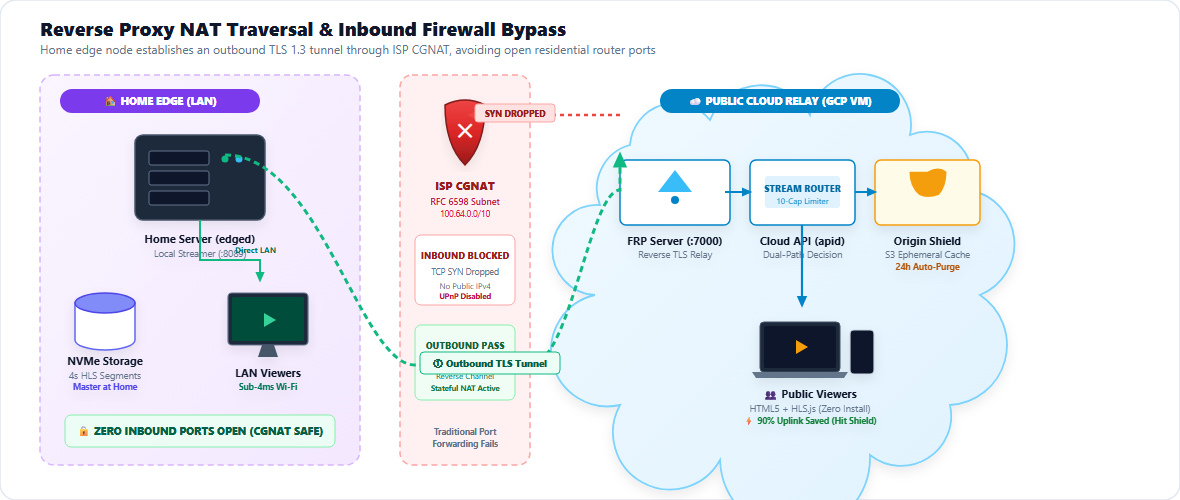
\includegraphics[width=0.98\textwidth]{figures/diag_01_nat_traversal.png}
\caption{Mechanics of Reverse Proxy NAT Traversal via Multiplexed Outbound Control Connections}
\label{fig:frp_tunnel_mechanics}
\end{figure}

As conceptualized in Figure~\ref{fig:frp_tunnel_mechanics}, reverse proxy tunneling inverts the connection initiation direction:
\begin{enumerate}
    \item The home edge node initiates an \textbf{outbound} TCP connection to the cloud relay server's public static IP address on port 7000. Because this packet originates from within the local network, the residential router and ISP CGNAT gateway classify it as legitimate outbound client traffic, dynamically creating a temporary bidirectional mapping in their state tables.
    \item The connection is upgraded to a mutually authenticated TLS 1.3 session \cite{rescorla2018transport}. Over this persistent control connection, the edge daemon and cloud relay negotiate a multiplexed tunnel using stream multiplexing protocols (e.g., Yamux).
    \item When an external cloud service or viewer requests a chunk from the edge, the request hits the cloud relay server. The relay maps the incoming virtual host or port to the active outbound control session established by that specific edge node.
    \item The request payload is framed and routed downstream across the existing multiplexed connection to the home node's local HTTP streamer, which serves the requested HLS chunk back up the tunnel without ever exposing an open inbound listening port on the home router.
\end{enumerate}
This theoretical framework provides the foundation upon which CustardFin's two-tier architecture is constructed and deployed.
